\documentclass[conference]{IEEEtran}
\IEEEoverridecommandlockouts
% The preceding line is only needed to identify funding in the first footnote. If that is unneeded, please comment it out.
\usepackage{cite}
\usepackage{amsmath,amssymb,amsfonts}
\usepackage{algorithmic}
\usepackage{graphicx}
\usepackage{textcomp}
\usepackage{xcolor}
\def\BibTeX{{\rm B\kern-.05em{\sc i\kern-.025em b}\kern-.08em
    T\kern-.1667em\lower.7ex\hbox{E}\kern-.125emX}}
\begin{document}

\title{BeFree\\}

\author{\IEEEauthorblockN{Ren Jiang}
\IEEEauthorblockA{\textit{Candidate No: 97247} \\
\textit{University of Bristol}\\
}
\and
\IEEEauthorblockN{Kevin Jolly}
\IEEEauthorblockA{\textit{Candidate No: 97249} \\
\textit{University of Bristol}}
}

\maketitle

\begin{abstract}
BeFree is an online community for football fans where
people bet on football matches, compete with other users
to earn points and write comments of football matches to communicate with each other. It is a serverless application hosted on Amazon Web Services and can be accessed at https://s3.eu-west-2.amazonaws.com/befree-uob/index.html. Source code of BeFree can be found at https://github.com/Jeaung/COMSM0010-Project.
\end{abstract}

\begin{IEEEkeywords}
Cloud Computing, Football Community, Amazon Web Services, Serverless
\end{IEEEkeywords}

\section{Introduction}
BeFree is an application where people can bet on football
matches without using money. Money is replaced here by
points which people can get by predicting correctly. Then,
they can climb up to the top of the rankings the better they
are at predicting scores. We also want to create an environment
where people can share their opinions about football by
posting comments. Our goal is to attract users from the huge football
fan base in the world (an estimated 4 billion people follow
football in the world).

When users sign up for BeFree, they will be initially
allocated a certain amount of points. Users will be able to bet
those points and the website will encourage them to compete
and communicate around football. Users can bet on several
aspects of a match such as the outcome of the match, the
number of goals scored, which players scored, etc. Each aspect
accounts when awarding points to users. The more points they
bet, the more they can win or lose at the end of the match.
In addition, there will be ranking lists after every match in
which users are ranked by the points they win or how well
their guesses are.

Users can also write comments and interact with each other
by liking or disliking others’ comments. They can earn points
by writing top comments on matches which have been liked
by other users. This procedure will facilitate users to interact
with each other and make them stick to the application.

\section{Cloudification}
We choose Amazon Web Services (AWS) \cite{b1} as our hosting platform for several reasons. Firstly, our system architecture is inspired by AWS Serverless Application Model (SAM) \cite{b2} which we believe is a trivial way to build a scalable system. Secondly, we are able to apply for AWS Educate free credits sufficient to build our project. Thirdly, AWS Cloudformation \cite{b3} provides the function of infrastructure as code so as a group of two, we benefit from it an easily reproducible infrastructure in group work.

\section{System Architecture}
Choosing to apply a serverless architecture is mainly because AWS SAM provides several benefits \cite{b2}. 
\begin{itemize}
\item Single-deployment configuration
\item Extension of AWS CloudFormation
\item Built-in best practices
\item Local debugging and testing
\item Deep integration with development tools
\end{itemize}

And bearing in mind the key of scalability, we make extensive use of existing services provided by AWS and push availability guarantee and scalability capability to AWS, the service provider, so that we only need to focus on building our core business logic.

\begin{figure}[htbp]
\centerline{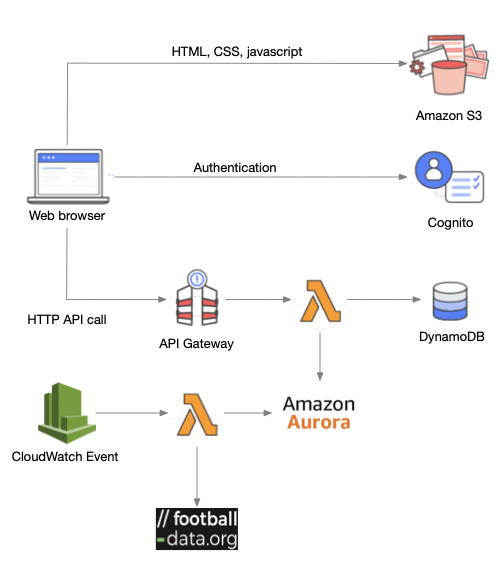
\includegraphics{architecture.png}}
\caption{System Architecture Overview}
\label{architecture}
\end{figure}

\subsection{Serverless}
All code is run in AWS Lambda \cite{b4} functions because Lambda takes care of server provisioning and management and offers auto-scalability and high availability which is very useful for the scalability of our system APIs. In BeFree, another usage of Lambda function is to pull football match data from 3rd party APIs routinely. We call it crawler function. This is done by configuring a CloudWatch \cite{b5} event using a cron expression to trigger the Lambda function periodically.

\subsection{Site Hosting}
BeFree employs AWS Simple Storage Service (S3) \cite{b6} to host its static website resources such as HTML, CSS, Javascript and images. When users visit our website, the web browser fetches web pages from S3 and Javascript code calls Lambda functions through API Gateway \cite{b7} and display data on the pages.

\subsection{User Management}
We adopt Amazon Cognito \cite{b8} to do user management and authentication since it's already a mature solution and saves us a lot of time.

\subsection{Database}
For databases, we use both Amazon DynamoDB \cite{b9} and Amazon Aurora \cite{b10}. DynamoDB is used to store typical key-value data such as comments and bettings. Amazon Aurora, as a relational database, stores match data and because we need flexible queries against matches such as date time, status or league. In addition, the queries does not provide a key so DynamoDB is inapplicable here (Its Scan does not meet demands either because the data needs to be sorted). The main advantage of using Amazon Aurora is that Amazon Aurora Serverless \cite{b11} allows it to automatically start up, shut down, and scale capacity up or down based on application's needs.

The reason for including DynamoDB instead of only using Aurora is that, for key-value data, DynamoDB outperforms Aurora with peaks of more than 20 million requests per second \cite{b9} while Aurora, as RDS, can only reach a maximum of about 200000 IOPS \cite{b12} \cite{b13}. Furthermore, in terms of pricing, in early stages, DynamoDB is basically free \cite{b14}. On the other hand, Aurora is charged by the hour as long as it's active \cite{b15}.

\section{Scalability}
Scalability remains a vital part in designing a web application and it means removing or mitigating system bottlenecks. Intuitively, bottlenecks of a system fall into two groups i.e. internal and external. Internal bottlenecks lie in both hardware (CPU, memory, network etc.) and software not being able to fully utilising the hardware resources. Because the number of AWS Lambda functions increases as system traffic grows, more hardware resource and software instances are created in isolation \cite{b14}. Thus, in BeFree, internal bottlenecks could be eliminated by Lambda's auto scaling.

On the other hand, external bottlenecks are the ones of the system's depending services. The directly depending services of BeFree are S3, Aurora, DynamoDB, API Gateway and Cognito. S3 hosts static web resources which users directly interact with. As claimed by AWS, s3 scales storage resources up and down to meet fluctuating demands so it's not a bottleneck of our system. Aurora, with its serverless configuration, can also seamlessly scale compute and memory capacity as needed, with no disruption to client connections. Again, this is not a bottleneck for scaling. Similar to Aurora Serverless, DynamoDB is said to be able to automatically scales tables up and down to adjust for capacity and maintain performance. According to its website, API Gateway creates, maintains, and secures APIs at any scale. Finally, Amazon Cognito User Pools provide a secure user directory that scales to hundreds of millions of users.

Overall, each component both internal or external of BeFree is fully managed by AWS and is able to auto-scale to some extent. So theoretically, BeFree has the capability to auto-scale infinitely as long as all of AWS's services are infinitely scalable.

We did some load testing against some of our representative APIs and below table shows the result.

TODO load testing


\section{Design and Implementation}
TODO could write about user walkthrough, betting and ranking design and implementation

\section{Future Work}
In the future, there are several aspects which we can improve.

Firstly, in our current architecture, web pages are not fully rendered before they are delivered to web browsers. Instead, Javascript code in web pages fetches data from our API and render them dynamically. Some search engines such as Baidu simply does not process Javascript in web pages \cite{b17}. Thus, our current approach is not search engine optimised so we may return the fully rendered pages to browsers in the future.

Secondly, we now only get football match data only from one 3rd party API, we plan to adapt several other APIs and add some retry strategies to our crawler function to improve data availability.

Thirdly, our home page serves to fetch and display match data from Aurora. Although Aurora Serverless is able to auto-scale, we could potentially cut down our cost and improve performance by introducing a cache layer using Amazon ElasticCache \cite{b18}. Compared to Aurora, ElasticCache with all the data in memory is able to respond in sub-millisecond time. However, extra complexity will arise because data consistency in ElasticCache and Aurora needs to be guaranteed.

\section{Conclusion}

\begin{thebibliography}{00}
\bibitem{b1} Amazon, “Amazon Web Services” https://aws.amazon.com/. Accessed: 2019-01-07.
\bibitem{b2} “AWS Serverless Application Model” https://docs.aws.amazon.com/serverless-application-model/latest/developerguide/what-is-sam.html. Accessed: 2019-01-07.
\bibitem{b3} “AWS Cloudformation” https://aws.amazon.com/cloudformation/. Accessed: 2019-01-07.
\bibitem{b4} “AWS Lambda” https://aws.amazon.com/lambda/. Accessed: 2019-01-07.
\bibitem{b5} “AWS CloudWatch” https://aws.amazon.com/cloudwatch/. Accessed: 2019-01-07.
\bibitem{b6} “Amazon Simple Storage Service” https://aws.amazon.com/s3/. Accessed: 2019-01-07.
\bibitem{b7} “Amazon API Gateway” https://aws.amazon.com/api-gateway/. Accessed: 2019-01-07.
\bibitem{b8} “Amazon Cognito” https://aws.amazon.com/cognito/. Accessed: 2019-01-07.
\bibitem{b9} “Amazon DynamoDB” https://aws.amazon.com/dynamodb/. Accessed: 2019-01-07.
\bibitem{b10} “Amazon Aurora” https://aws.amazon.com/rds/aurora/. Accessed: 2019-01-07.
\bibitem{b11} “Amazon Aurora Serverless” https://aws.amazon.com/rds/aurora/serverless/. Accessed: 2019-01-07.
\bibitem{b12} “Amazon RDS for MySQL, Fast, predictable storage” https://aws.amazon.com/rds/mysql/\#Fast.2C\_predictable\_storage. Accessed: 2019-01-07.
\bibitem{b13} “Amazon Aurora Features: MySQL-Compatible Edition, High Performance and Scalability“ https://aws.amazon.com/rds/aurora/details/mysql-details/\#High\_Performance\_and\_Scalability. Accessed: 2019-01-07.
\bibitem{b14} “Amazon DynamoDB Pricing“ https://aws.amazon.com/dynamodb/pricing/on-demand/\#DynamoDB\_free\_tier. Accessed: 2019-01-07.
\bibitem{b15} “Amazon Aurora Pricing“ https://aws.amazon.com/rds/aurora/pricing/. Accessed: 2019-01-07.
\bibitem{b16} “Understanding Container Reuse in AWS Lambda“ https://aws.amazon.com/blogs/compute/container-reuse-in-lambda/. Accessed: 2019-01-07.
\bibitem{b17} Bartosz Góralewicz, “Going Beyond Google: Are Search Engines Ready for JavaScript Crawling \& Indexing?“ https://moz.com/blog/search-engines-ready-for-javascript-crawling. Accessed: 2019-01-07.
\bibitem{b18} “Amazon ElasticCache“ https://aws.amazon.com/elasticache/. Accessed: 2019-01-07.
\end{thebibliography}
\vspace{12pt}

\end{document}

